\documentclass[a4paper]{article}

\usepackage{graphicx}
\usepackage{inputenc}
\usepackage{latexsym}

% \VignetteIndexEntry{signalextraction}

\title{Case Study on the Direct Filter Approach}
\author{Marcel Dettling and Marc Wildi}

\usepackage{c:/Programme/R/share/texmf/Sweave}
\begin{document}

\maketitle

\section{Purpose of the signalextraction-Package}

In general, a time series may be viewed as an aggregate of various
parts: for example trend plus seasonal plus noise component. Since
users are often interested in particular components only (for example
the trend or the seasonally adjusted time series), filters are used to
`remove' the undesirable ones. \\

In practice, signal extraction is based on finite samples
$X_1,...,X_T$ and, very often, \emph{current} estimates of the
interesting components ($t=T$) import: a so-called `concurrent' or
`real-time' estimate of the trend or of its turning-points has a
strong prospective content, since the future evolution of the time
series is likely to be conditioned by this component. Whereas
forecasting tools generally emphasize the one-step ahead perspective
(at least this is true for model-based approaches such as ARIMA),
real-time signal extraction may be used to infer future mid-term
dynamics. \\

The following package proposes real-time signal extraction algorithms
based on Wildi \cite{wildi2007}. In the following, references to the
book are marked by an asterisk $^*$ in the text. The main difference
between traditional model-based approaches (such as ARIMA) and the
direct filter approach (dfa) is that the latter optimization criteria
emphasize specifically two important estimation problems: the
estimation of the \emph{current level} (of the interesting signal) and
the \emph{early detection of turning-points} (of a trend component). 
Since both criteria are incongruent, different algorithms are
available which match user preferences (level or turning-points) and
time series characteristics (trending or non-trending series). Also,
important filter characteristics at frequency zero can be imposed or
relaxed such as the \emph{local level
  restriction}\footnote{\label{foot1}$A(0)=1$, where $A(\omega)$ is
  the amplitude function.} or the \emph{instantaneous level
  restriction}\footnote{$A(0)=1$ and the time delay of the filter
  vanishes in frequency zero.}. \\

This document provides a `step-by-step' introduction to the dfa
real-time signal extraction package and demonstrates its
functionalities based on a leading indicator application (the
so-called KOF-Economic Barometer). More generally, the text emphasizes
topics that are specific to real-time signal extraction. 

\section{Data Import}

The starting point to the case study in this chapter is a time series
with at least 61 monthly or 23 quarterly entries. A very common case
is that the data are present in a column of a spreadsheet, as
displayed in Figure 1. We will thus start our tutorial from there. 

\begin{figure}[h!] 
\begin{center}
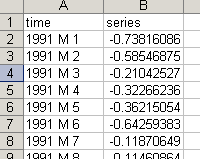
\includegraphics{excelneu}
\caption{A time series with measurement time information and
  informative headers stored in a spreadsheet. Row A contains
  the headers \emph{time} and \emph{series}, column A information
  about when the measurements were made and column B is the series
  itself.} 
\end{center}
\end{figure}

How can we get such data from a spreadsheet into R? We here recommend
a straightforward way: first, save the data from the spreadsheet
software as a tab-delimited text file named \texttt{series.txt}. 
Second, read them from the text file into R and process them
accordingly. Only three simple commands are necessary. 

\begin{verbatim}
> input <- read.delim("series.txt")
> x     <- as.numeric(input$series)
> names(x) <- input$time
\end{verbatim}

Please note that the above commands only work if the configuration in
the spreadsheet is exactly as displayed in Figure 1. In particular,
the first line of code contains the text file name/path and needs to
be set/chosen accordingly. The case where there is no header row can
be dealt with by setting the argument \texttt{header=FALSE} in the
\texttt{read.delim()} function. On the other hand, if column A with
the times of measurement is not present, the last of the three lines
of code in the above chunk gets obsolete. Further information about
how to read external text files into R is available from the manual
page of the import function \texttt{read.delim}, which can be called
by

\begin{verbatim}
> help(read.delim)
\end{verbatim}

\section{Business Survey Data}

In fact, the business survey dataset \texttt{x} that we just generated
is already present as an example dataset in the
\texttt{signalextraction}-package. Reading it from a text file is thus
not strictly necessary (and was done here for illustrative purposes
only), as it can conveniently be loaded into R via

\begin{verbatim}
> data(x)
\end{verbatim}

This series is a monthly index of business survey data with 183
measurements between January 1991 and March 2006. It is used by the
Swiss Institute for Business Cycle Research to anticipate movements of
the GDP growth rate. For an analysis, we employ the direct filter
approach that is implemented in the \texttt{signalextraction}-package
by the \texttt{dfa()}-routine. The default call is

\begin{verbatim}
> dfa <- function(x, quart = FALSE, d = 0, pb = 1/14, sb = 1/7,
                  tpfilter = FALSE, lambda = 3, expweight = 1.5, 
                  pbd = if (length(x)<100) 1.08 else 1.03, 
                  limamp = if (!tpfilter) 1.5 else 3, i2 = TRUE, 
                  n.loops = 10, verbose = 1)
\end{verbatim}

The first three arguments \texttt{x}, \texttt{quart} and \texttt{d}
describe the time series and their properties. We are going to work
with the business survey data that we read/loaded into R before. 
Argument \texttt{quart} describes whether the series was recorded with
monthly or quarterly frequency. As evident from Figure 1, we have
monthly measurements for our series and thus use the default value
\texttt{quart=FALSE}. \textbf{Please note: the present version of the
  package has been tested with monthly data only!} \\

Argument \texttt{d} is related to the determination of the
optimization criterion and of filter constraints, see sections $6.1^*$
and $6.2^*$ (ref: Wildi \cite{wildi2007}). Roughly, one can say that
for stationary or asymptotically bounded time series (as is the case
for the business survey data \texttt{x}) \texttt{d}=0 is the right
choice whereas for trending series \texttt{d}=1 would be more
appropriate. \\

Setting \texttt{d=1} imposes a local level restriction (see footnote
\ref{foot1}). A formal test verifying the necessity of imposing
\texttt{d=1} is proposed in chapter $6^*$, where it is shown, also,
that the proposed procedure can be interpreted as a generalization of
traditional unit root tests. In particular, \texttt{d=1} should be set
for integrated processes. It should be emphasized, however, that
filter constraints and the optimal selection of optimization criteria
determined by \texttt{d} address issues that extend the concept of
integration, see for example sections $6.6^*$ and $6.7^*$. \\

For \texttt{d=0}, the optimization is based on criterion $3.7^*$
(periodogram) and the amplitude function $A(\omega)$ of the one-sided
filter is not constrained to satisfy $A(0)=1$\footnote{See section
  $4.5^*$ for a thorough discussion on these topics.}, see for example
the bottom left panels in Figures \ref{fig1} and \ref{fig2}. For
\texttt{d=1}, the optimization is based on criterion $6.7^*$
(pseudo-periodogram) and the amplitude function of the one-sided
filter is constrained by requiring $A(0)=1$\footnote{Altough the
  constraint $A(0)=1$ could be obtained by a simple scaling of the
  filter \emph{after} optimization, it is better to impose it
  \emph{during} the optimization process. As a consequence, this
  restriction entails filter performances more fundamentally by
  affecting the location of poles and zeroes directly.}. \\

The remaining arguments in the call of \texttt{dfa()} are described
next. 


\section{Signal}\label{sect3}

Any signal can be approximated by optimal one-sided
ZPC-filters\footnote{See section $3.2^*$ for a formal definition of
  the latter filter class.} used in the package. For our purpose, we
have found the so called `ideal' trend to be a very convenient
target-signal.  The transfer function of the ideal trend is defined by
\begin{eqnarray}
\label{tfile} {\Gamma}(\omega):=\left\{\begin{array}{lr}1&0\leq|\omega|\leq\pi 
\cdot pb \\ \displaystyle{\frac{\pi \cdot sb-|\omega|}{\pi \cdot sb-\pi \cdot 
pb}}~~&\pi \cdot pb\leq|\omega|\leq\pi \cdot sb\\ 0&\pi \cdot sb\leq|\omega|
\leq\pi\end{array}\right. 
\end{eqnarray}
where \texttt{sb} and \texttt{pb} (\texttt{pb} $<$ \texttt{sb}) are
parameters in the above function-call: \texttt{pb} determines the
width of the pass-band and \texttt{sb} determines the width of the
stop-band. They can take values in $(0,1)$, corresponding to the
frequency band $(0, \pi)$. For our own applications we set
\texttt{pb}< \texttt{sb}< 1/6, which ensures that seasonal components
are eliminated. 

In-between \texttt{pb} and \texttt{sb}the transfer function decays
linearly from pass- to stop-band. Strictly speaking, this signal
cannot be computed exactly because it is the output of a
doubly-infinite MA-filter.  Moreover, at the current boundary $t=T$ of
$X_1,...,X_T$ a one-sided
filter must be used necessarily. \\

\begin{quote}The function \texttt{dfa()} computes real-time
  (concurrent) one-sided filters whose output approximates the current
  level of the signal (see section \ref{levapp} below) or for
  detecting turning-points of the trend (see section \ref{section5}
  below).\end{quote}


\noindent By choosing smaller \texttt{pb} and \texttt{sb}, the target
(trend) signal becomes smoother implying that its real-time
approximation, through \texttt{dfa()}, will as well become smoother in
general. The default values \texttt{pb=1/14}, \texttt{sb=1/7} in the
above function-call have been determined in the context of
business-cycle analysis and are, to some extent,
arbitrary\footnote{\texttt{sb=1/7} implies that components with
  frequency equal or greater to $\pi/7$ are eliminated by the ideal
  trend. Note that the first (fundamental) seasonal frequency is
  $\pi/6$.}.\\

It is up to the user to determine which signal best fits its
particular purpose: an intra-day trader would prefer short-term trends
while a climatologist would be interested in long-term variations. 
Ultimately, these parameters map user preferences to the (statistical)
optimization algorithms which is impossible if signals are determined
by automatic modeling procedures such as implemented in traditional
model-based approaches. 

Thus, the use of alternative target signals is possible, but this
additional flexibility has not been implemented in the package yet. 
Nevertheless, the user can substitute the `ideal' trend by a signal of
its own by a simple source code manipulation. More precisely, one has
to change a vector called \texttt{ttr} in \texttt{dfa()}: one can
search for the following piece of code
\begin{verbatim}
    ## Symmetrical transfer function
    ttr       <- as.numeric(((1:(npg2+1)) <= npg2*sb))
    weli      <- floor((npg2*sb+1):(npg2*pb+1))
    term1     <- npg2*sb+1-((npg2*pb+1):(npg2*sb+1))
    ttr[weli[1]+weli[length(weli)]-weli] <- term1/(npg2*sb-npg2*pb)
\end{verbatim}
and replace the values in \texttt{ttr}\footnote{A plot of ttr would
  reveal that it corresponds to the transfer function of the ideal
  trend (restricted to positive frequencies only). More precisely,
  ttr[i] corresponds to the value of the (intended) transfer function
  in frequency $\omega_i:=(i-1) \cdot \pi/(L-1)$ whereby $L$ is the
  length of ttr: therefore $\omega_1=0$ and $\omega_L=\pi$.} by
(almost) any other (transfer) function. \\

It is worth to emphasize that the present version of the package has
been developed with trend-estimation in mind. It is best suited for
approximating low-pass filters. \emph{The optimization procedure is
  not optimally designed for high- or band-pass applications}
(although this could be implemented of course) because of particular
initial value settings and fixed filter constraints. 




\section{Level-Approximation}\label{levapp}

In analogy to \texttt{d}, the argument \texttt{tpfilter} is a very
crucial input for the signal extraction, since it preselects the
optimization criterion that is employed. For the default value,
\texttt{tpfilter=FALSE}, we are in the case of level-estimation, see
chapters $3^*$, $4^*$ and $6^*$. This means that the
\texttt{dfa()}-routine fits a best level filter, i.e.  tries to track
the trend signal as closely as possible, without a special focus on
turning points.\\

\noindent By setting \texttt{tpfilter=FALSE}, two level-specific
optimization criteria can be accessed :
\begin{itemize}
\item For \texttt{d=0} criterion $3.7^*$ is used (best suited for
  stationary or asymptotically bounded time series). 
\item For \texttt{d=1} criterion $6.7^*$ is used (pseudo-periodogram)
  and $A(0)=1$ is imposed (low-pass filter). 
\end{itemize}
\begin{figure}[htb!] 
\begin{center}
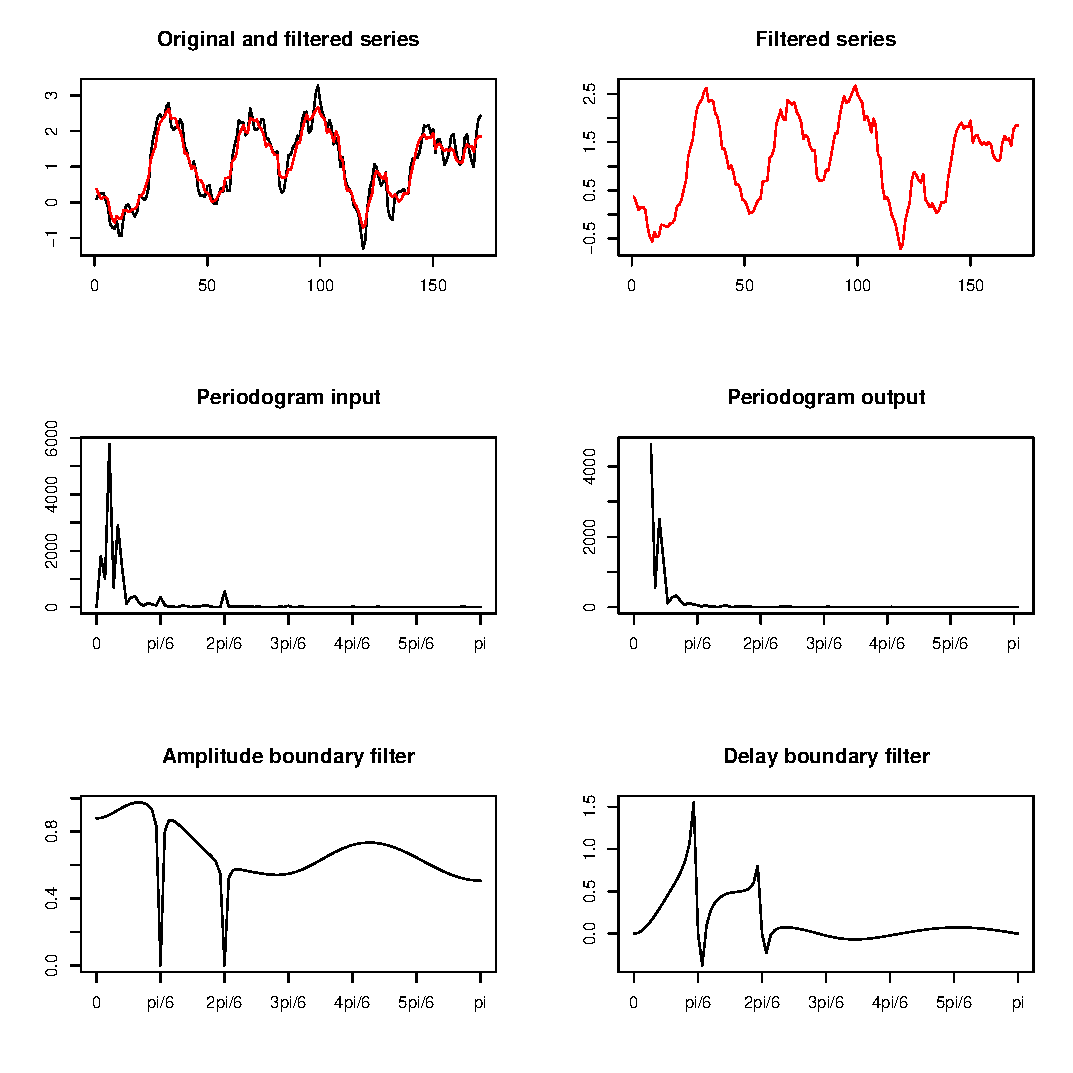
\includegraphics{levelfilter_la5_exp2k5_pbd1k02_pb_14_sb7_limamp5_nloops10_d0}
\caption{Graphical output after a signal extraction using the
  \texttt{dfa()} routine for best level estimation (with default
  arguments) on the business survey data \texttt{x}. The top two
  panels show the original and filtered time series, the middle two
  periodogram input and output, and the bottom two amplitude and time
  shift characteristics of the one-sided filter.\label{fig1}}
\end{center}
\end{figure}
Let us now run the direct filter approach with default arguments (thus
they are not visible in the call) which implies best level
approximation. The command is as follows:
\begin{verbatim}
> fit <- dfa(x)
\end{verbatim}
\emph{Note that the numerical optimization algorithm may need some
  time to complete: progress can be viewed in the R-window}. 
Technically, we obtain a R-object named \texttt{fit}. It is an
instance of class \texttt{dfa}, for which (among others) a plot method
has been defined. It is called by
\begin{verbatim}
> plot(fit)
\end{verbatim}
and yields a 3\texttt{x}2 panel of 6 diagnostic diagrams, see Figure
2. The top left plot shows an overlay of the business survey series
\texttt{x} (black) with the filter output (red). The two panels in the
middle show the periodogram input and output: this is a very
convenient way to check whether the filter has removed (damped)
undesirable components in the original time series or not. Finally,
filter characteristics such as \emph{amplitude} and \emph{time
  shift}\footnote{The time shift function is simply the phase divided
  by frequency, see $2.9^*$.} functions can be viewed in the bottom
panels, see chapter $3^*$ for an overview on filter characteristics in
the frequency-domain. 



\section{Turning Point Detection}\label{section5}

In the following, turning-points are defined as local extrema of the
ideal trend, see section $5.1^*$ for a more comprehensive discussion
about these topics. Therefore, altering the signal definition (through
\texttt{pb} and/or \texttt{sb}) affects the turning-points, too.\\


If turning points are of interest, then argument \texttt{tpfilter}
should be set to \texttt{tpfilter=TRUE} in the function call. As a
consequence, the error criterion optimized by \texttt{dfa()} is the
one in equation $5.4^*$. We also strongly recommend to set
\texttt{d=0} and \texttt{i2=TRUE} which is the standard configuration
(more on these below). \\

The filter output in Figure \ref{fig2} has been obtained by using the following function call:
\begin{verbatim}
> fit <- dfa(x, quart = FALSE, d = 0, pb = 1/6.5, sb = 1/6, 
             tpfilter = TRUE, lambda = 5, expweight = 1.5, 
             pbd = 1.02, limamp = 3, i2 = TRUE, n.loops = 10, 
             verbose = 1)
>
> plot(fit)
\end{verbatim}

\begin{figure}[h!] 
\begin{center}
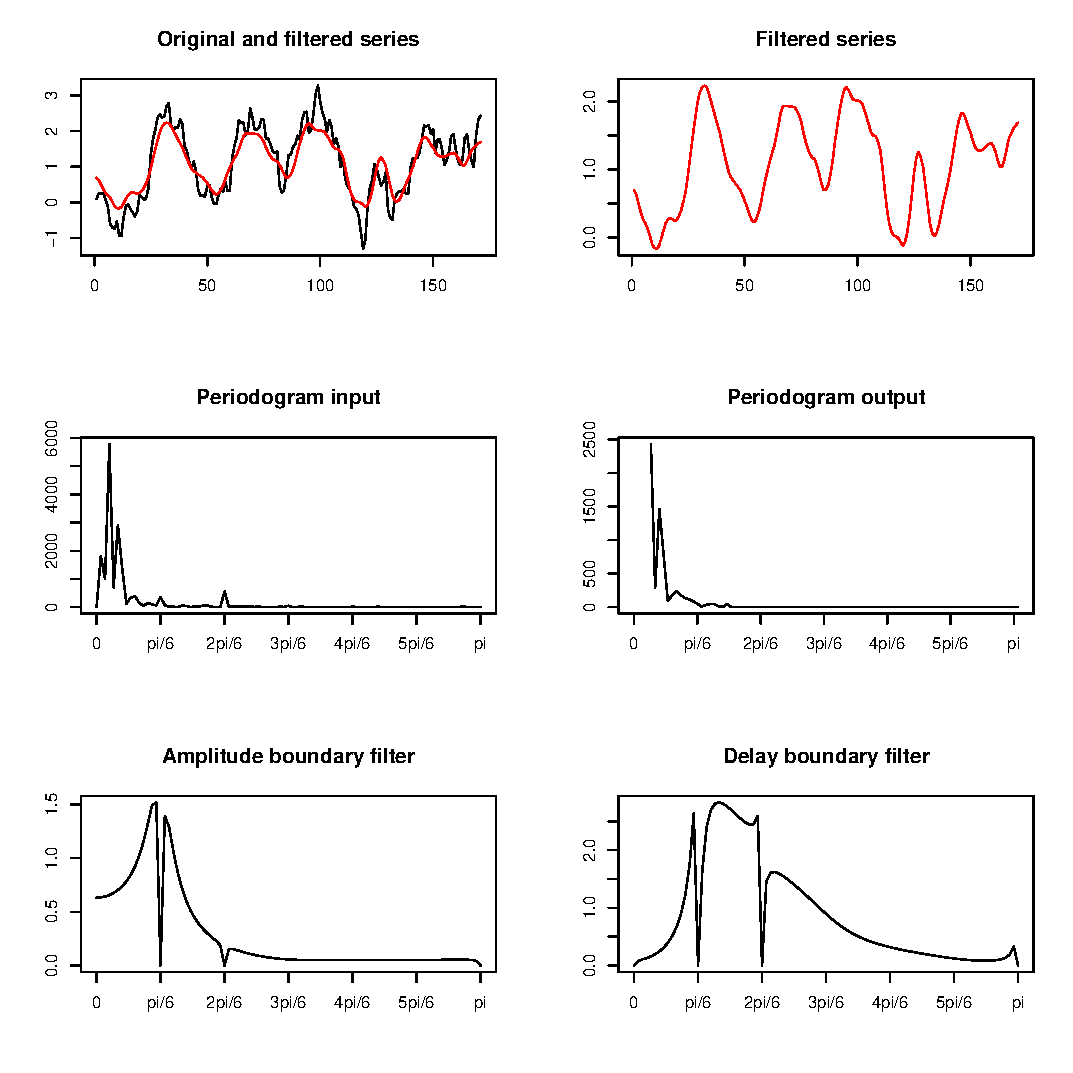
\includegraphics{tpfilter_la5_exp1k5_pbd1k02_pb_6k5_sb6_limamp5_nloops10_d0}
\caption{Graphical output after a signal extraction using the
  \texttt{dfa()} routine for turning point detection. The top two
  panels show the original and filtered time series, the middle two
  periodogram input and output, and the bottom two amplitude and time
  delay boundary filters.\label{fig2}}
\end{center}
\end{figure}

Before motivating this particular choice (parameter-setting) we note
that the output series is much smoother than for the previous level
estimate. Level performances are generally worse but turning-points
are detected very early and the enhanced smoothness ensures that the
rate of `false alarms' is small, see chapter $5^*$\footnote{Empirical
  comparisons of turning-point filters, level filters and logit-models
  are shown in section $5.3.2^*$.}. The smoothness is due to stronger
damping of undesirable high-frequency components in the stop-band and
the improved speed is obtained by very small time delays in the
pass-band, as confirmed by the bottom panels in
Figure \ref{fig2}\footnote{A comparison with filter characteristics of
  the level-filter in Figure \ref{fig1} illustrates that the damping
  effect of the turning-point filter is much stronger in the stop-band
  and that the time delay is barely larger in the pass-band (in
  particular in the vicinity of the low-frequency spectral bulk).}.\\

\begin{quote}It is worth to emphasize that filter-outputs obtained by
  \texttt{dfa()} are not subject to revisions (as would be the case
  for traditional model-based approaches) because causal (one-sided)
  filters are used only. \end{quote}

\section{Other Arguments to dfa()}

While it is far beyond the scope of this document to display or
discuss the results with all possible combinations in the
multi-dimensional space of the arguments \texttt{lambda},
\texttt{expweight}, \texttt{pbd}, \texttt{pb}, \texttt{sb},
\texttt{limamp} and \texttt{i2}, we will shed light on some of the
most important aspects:
\begin{itemize}
\item \texttt{lambda} is a Lagrange parameter for phase restriction,
  where larger values induce smaller time delays in the pass-band of
  the filter, but noisier signal estimates. It emphasizes the filter
  error due to the time delay in the generalized criterion $5.4^*$. 
\item \texttt{expweight} is a parameter that determines the shape of
  the frequency weighting function $W(\omega)=|\omega|^{expweight}$ in
  criterion $5.4^*$. Larger values emphasize damping efforts in the
  stop-band of the filter. For \texttt{lambda}=1 and
  \texttt{expweight=0} the best level filter results. Emphasizing
  simultaneously the time delay (in the pass-band), through
  \texttt{lambda}, and the amount of high-frequency (noise) damping in
  the stop-band, through \texttt{expweight}, generates distortions of
  the amplitude function in the pass-band which are associated to
  poorer level performances, see section $5.3^*$, for a comprehensive
  discussion on these topics. In particular, it is shown that the
  detection of turning points and the approximation of the level (of
  the signal) are to some extent incongruent criteria which require
  specific solutions provided in \texttt{dfa()}. 
\item \texttt{pbd} implements a regularity constraint which must
  exceed one. Roughly speaking, the shorter the time series, the
  larger \texttt{pbd} should be set (see section $10.5^*$ for
  details). More precisely, \texttt{pbd} is the value that the moduli
  of poles of the ARMA filter are constrained to exceed, see $3.20^*$,
  and therefore it ensures stability of the resulting one-sided
  filter. The larger it is, the smoother the transfer function usually
  is (which does not mean that the output signal will be smoother, of
  course). So far, we have found that \texttt{pbd}=1.08 is a good
  choice if $T<100$ whereas if $T>100$ ony may set \texttt{pbd}=1.03,
  see $3.20^*$ (deviations are possible, of course). 
\item In the case of turning-point filters, the amplitude in the
  pass-band may be subject to more or less severe distortions. The
  parameter \texttt{limamp} enables to limit the extent of such
  distortions. More precisely, the parameter constrains the amplitude
  $A(\omega)$ to be smaller than $limamp*A(0)$ in the pass-band of the
  filter: this amounts to a particular (additional) regularity
  constraint. The parameter should be larger than one. From a
  practical point of view, we have found that values between 1.5 and 2
  are fine in the case of level approximation
  (\texttt{tpfilter=FALSE}) whereas values between 3 and 5 are
  reasonable constraints in the case of turning-point filters. 
\item \texttt{i2} is a logical which determines whether the time delay
  of the one-sided filter vanishes at frequency zero (default-value
  \texttt{i2=TRUE}) or not. If \texttt{i2=TRUE} and \texttt{d=1} then
  an \emph{instantaneous level restriction} is imposed, see section
  $6.2.1^*$: it is shown that this constraint can be associated to
  processes whose trend-slope grows unboundedly in absolute value such
  as, for example, I(2)-processes. However, as for \texttt{d}, the
  scope of \texttt{i2} transcends `integration orders'. If
  \texttt{i2=TRUE}, then the constraint is implemented formally by
  using an additional zero-pole pair satisfying $6.12^*$. In practice,
  we have found evidence that this constraint is often useful (whether
  series are integrated or not), in particular if turning points are
  of interest. Empirical results in chapter $4^*$ suggest that level
  performances are enhanced also by imposing this restriction. Note
  that the analyzed series there are asymptotically bounded (and thus
  cannot be I(2)) which illustrates that methodological issues related
  to the values of \texttt{i2} or \texttt{d} (i.e. the choice of
  corresponding optimization criteria and/or filter restrictions)
  encompass model assumptions such as `integration' (see the
  discussion in sections $6.6^*$ and $6.7^*$). 
\end{itemize}

\noindent In order to illustrate the effect of the above parameters we
compare filter outputs obtained by alternative settings:
\begin{itemize}
\item Black line in Figure \ref{fig4}: the series is based on the
  original setting, whose outcome was already plotted in Figure
  \ref{fig2}. 
\item Red line in Figure \ref{fig4}: the series is based on
  \texttt{expweight=0.5} (instead of 1.5), everything else being equal
  to the original setting. The smaller weight ($|\omega|^{0.5}$
  instead of $|\omega|^{1.5}$ in the original setting) attributed to
  the `undesirable' high-frequency components in criterion $5.4^*$
  implies that damping properties of the filter in the stop-band
  aren't emphasized as strongly as in the original setting. Therefore,
  the resulting filter output is contaminated by high-frequency
  `noise' which makes an assessment of turning-points (in real-time) a
  more difficult task in practice. 
\item Blue line in Figure \ref{fig4}: the series is based on
  \texttt{lambda=2} (instead of \texttt{lambda=5}), everything else
  being equal to the original setting. The filter output is close to
  the black-line. However, the smaller lambda-weight attributed to the
  time-delay in criterion $5.4^*$ generates a filter which is slightly
  delayed (a closer look at the figure reveals that the delay with
  respect to the black line is approximately one month). 
\item Green line in Figure \ref{fig4}: the series is based on
  \texttt{lambda=2} and \texttt{pb=1/15}, \texttt{sb=1/13}. The filter
  output is smoother and it is delayed. Note that the signal has
  changed by choosing \texttt{pb=1/15}, \texttt{sb=1/13}, recall
  section \ref{sect3}. Therefore, turning-points have changed too. 
  Strictly speaking, the green line should not be compared to the
  preceding ones because the optimal signal has been altered. 
\end{itemize}

\begin{figure}[htb!] 
\begin{center}
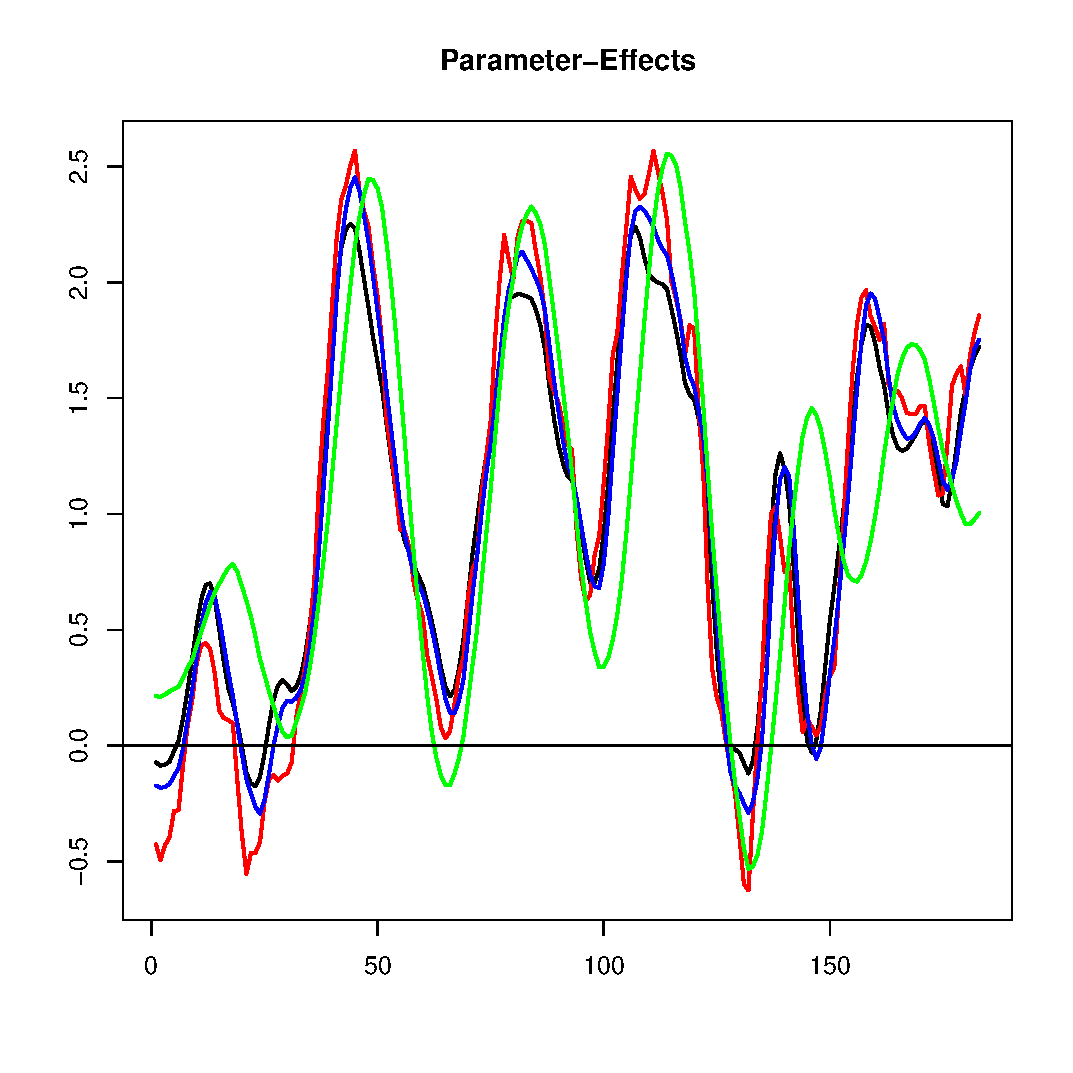
\includegraphics{parametersetting}
\caption{Effect of various parameter-settings on filter
  outputs\label{fig4}}
\end{center}
\end{figure}

Regarding the influence of the filter arguments, one should note that
\texttt{lambda} and \texttt{expweight} have no effect on the output
for best level estimation, i.e. if \texttt{tpfilter=FALSE}. However,
\texttt{d}, \texttt{pbd}, \texttt{pb}, \texttt{sb}, \texttt{limamp}
and \texttt{i2} can be set. 







\section{Numerical Optimization Routine}

Minimizing the error criteria given in $3.7^*$, $5.4^*$ or $6.7^*$ is
a difficult, highly non-linear problem that cannot be solved
explicitly and requires a numerical approach\footnote{The standard
  optimization routines implemented in R are used: stochastic
  annealing, Nelder-Mead and BFGS.}. As always in numerics, there is a
trade-off between the accuracy of the solution and the required
computing time.  In \texttt{dfa()}, this is governed by argument
\texttt{n.loops}, which corresponds to the number of initial
Stochastic Annealing proposals that are drawn, and then further
optimized by a variety of numerical optimization methods. The more of
them we use, the smaller the chance of being trapped in local extrema
becomes, but the computing gets more time consuming.  To our
experience, the default value \texttt{n.loops=10} balances computing
load and precision reasonably well, and yields accurate solutions with
an average running time of around 2-3 minutes. \\

Finally, argument \texttt{verbose} controls the amount of text output
that is given during the numerical optimization. Three levels are
available: 0 corresponds to no output at all, the default value 1
allows for a rough guess which percentage of the computing has been
done, while a value of 2 yields full text output for every
optimization step and is mainly useful for debugging and exact
comparisons.\\

Since the numerical optimization partly relies on stochastic
algorithms it is possible that the same initial parameter-setting may
lead to slightly different solutions, depending on which draw is used
during optimization. While we did not find significant departures for
level-estimation problems, turning-point filters may be sensitive to
such issues because the optimization problem is `harder' to solve.\\


Storing and loading \texttt{dfa}-objects is possible with
\begin{verbatim}
> save(fit,file="myfile.rda")
> load("myfile.rda")
\end{verbatim}
where \texttt{myfile.rda} is a file-name. This enables to circumvent
laborious optimizations and to access more rapidly to `old' results.\\


\noindent \textbf{Every suggestion for improving the speed and/or the
  precision of the numerical optimization algorithm would be greatly
  appreciated!} It should be noted, however, that the problem is
technically more complex (less `regular') than traditional `amplitude
fitting' common in engineering applications. In particular, optimal
turning-point filters are likely to approach the frontier of
regularity (they are prone to become nearly singular) because the
amplitude function in the pass-band is to some extent `sacrificed' at
the benefits of smaller time delays (in the pass-band) and stronger
damping of high-frequency `noise' (in the stop-band). 




\section{Out-of-Sample Utilization of the Filter}

Behind the scenes, the direct filter approach computes a one-sided
ARMA-filter. The ARMA-coefficients are also stored in object
\texttt{fit}, from where they can be accessed by

\begin{verbatim}
> fit$ar.coef
 [1]  1.0000e+00 -1.7595e+00  1.6305e+00 -2.1317e-01 -1.0193e+00
 [6]  1.5434e+00 -8.9463e-01  1.3691e-01  4.0717e-01 -2.8254e-01
[11]  8.0379e-02  5.9704e-03 -8.9685e-04 -3.9952e-04 -4.1361e-05
[16] -1.7538e-06
>
>
> fit$ma.coef
 [1]  0.12004985 -0.08212789 -0.02056278  0.16565752 -0.06297009
 [6]  0.04579233  0.03375345 -0.00358081  0.02689532  0.02600401
[11]  0.02158400 -0.02785126 -0.01723218  0.04432262  0.01160852
[16] -0.05509042
\end{verbatim}
As an alternative, there is a method for the \texttt{dfa}-class that
extracts the coefficients directly. It is called by
\begin{verbatim}
> coef(fit)
      AR-coefficients MA-coefficients
 [1,]    1.000000e+00     0.120049851
 [2,]   -1.759552e+00    -0.082127897
 [3,]    1.630578e+00    -0.020562783
 [4,]   -2.13...          ... 
\end{verbatim}
\begin{figure}[htb!] 
\begin{center}
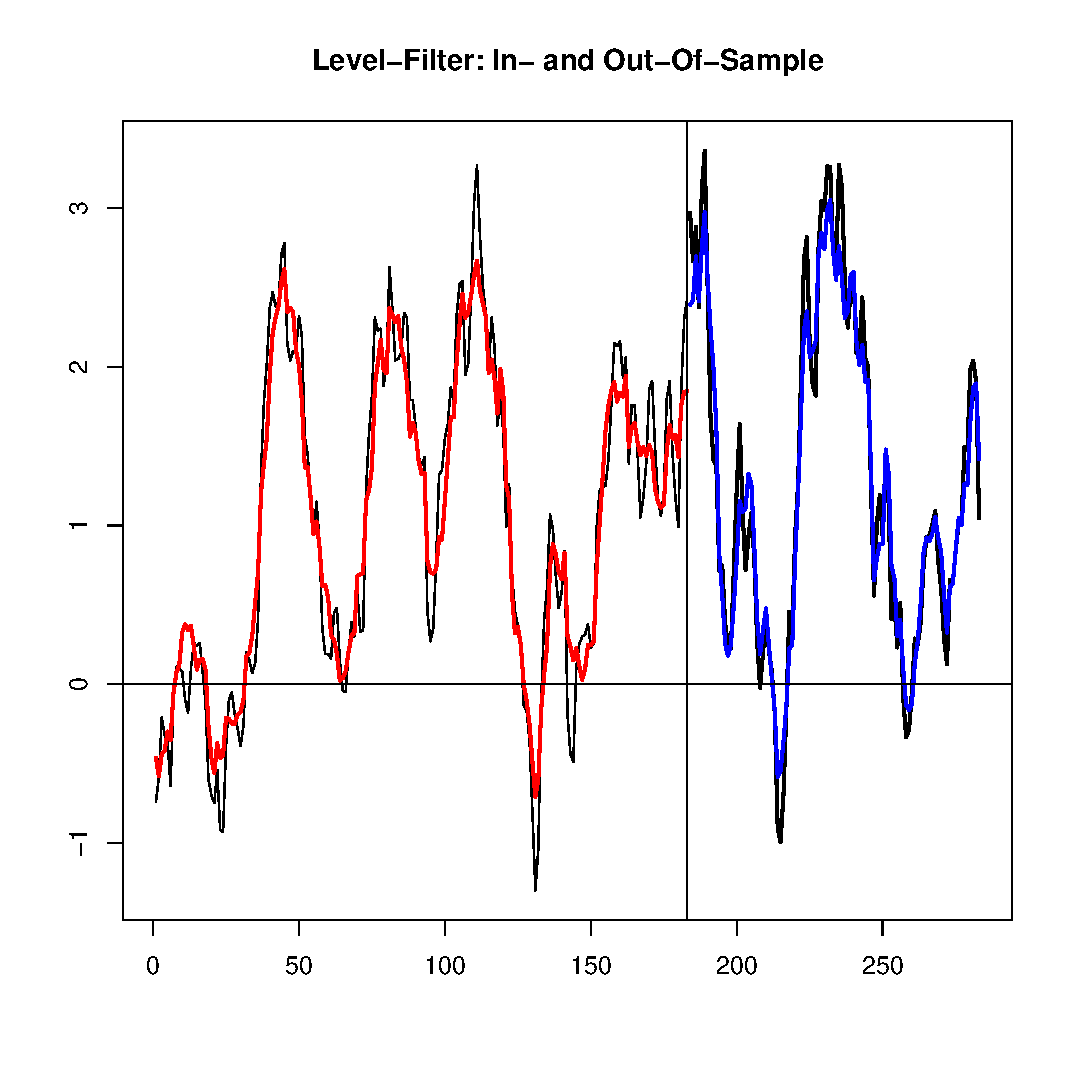
\includegraphics[width=1.5\textwidth]{level_in_and_outofsample}
\caption{Level filter that was estimated on the business survey data
  (observations 1-183, filter values are in red) and then applied to a
  simulated series with similar mathematical properties (observations
  184-283, filter values are in blue).\label{fig5}}
\end{center}
\end{figure}
and yields a matrix with two columns, where the first one contains the
AR- and the second one the MA-parameters. These coefficients can now
in principle be used for filtering any arbitrary time series. 
However, it is important to note that this is reasonable only if the
original and new series originate from a common probability
distribution, or in colloquial language, if they have ``the same
mathematical properties''. \\

The most convenient way to apply a previous filter to a new time
series is with the \texttt{outsamp}-method that is associated to the
\texttt{dfa}-class. It takes an arbitrary series as input and computes
the filter value for every datapoint. Or in other words, for every
datapoint in the new series, a nowcast of the trend signal is
computed, based on parameters that were estimated from another time
series. Such functionality also allows for easy performance
comparisons among different filter methods.\\

For an illustration of the \texttt{outsamp}-method, we here simulate a
time series that can be interpreted as a sequel to the business survey
data \texttt{x}. We do this by expanding an AR(13)-model that was
fitted to \texttt{x}. The commands are as follows. 

\begin{verbatim}
> set.seed(21)
> fit.ar <- ar(x)
> p      <- fit.ar$order
> innov  <- rnorm(100, sd=sqrt(fit.ar$var.pred))
> xx     <- c(rev(x)[1:p], rep(0,100))
> for (i in 1:100)
+   {
+     xx[i+p] <- sum(xx[i:(i+p-1)]*rev(fit.ar$ar))+innov[i]
+   }
> newx <- xx[(p+1):length(xx)]+mean(x)
\end{verbatim} % $

We employ the last 13 observations of \texttt{x} as starting values
for the new series and then generate 100 new datapoints by using the
AR(13)-model fitted on \texttt{x} with randomly drawn white noise
innovations, whose variances are equal to the error variance on the
business survey data. After doing so, we propose that the
distributions of \texttt{x} and the new series \texttt{newx} are
similar enough to justify an out-of-sample application of the filter. 

\begin{verbatim}
> blf  <- outsamp.dfa(fit, newdata=newx, sequel=TRUE)
\end{verbatim}
The resulting series (in the object \texttt{blf}) corresponds to the
blue line in Figure \ref{fig5}.\\

Note that there is an argument \texttt{sequel} that requires some
explanation: since behind the scenes, \texttt{dfa()} fits an
ARMA-ZPC-filter, we would in theory need an infinitely long series for
an exact computation of the filter values.  If the coefficients of the
MA($\infty$)-representation of the filter decay reasonably quickly
(which they do in most cases), this issue can be neglected. However,
at the beginning of the new series \texttt{newx}, we need to know from
which basis the filter values have to be computed or, in other terms,
we need starting values for initializing the AR-part of the filter. In
our case, where \texttt{newx} is a direct sequel to \texttt{x}, we set
argument \texttt{sequel=TRUE}. In this case, the past values which are
required to compute the nowcast are taken from the ``old'' series
\texttt{x}. On the other hand, if the values from the old series
cannot serve as initial values, the set argument
\texttt{sequel=FALSE}. The nowcasts at the beginning of \texttt{newx}
will then be determined on the basis of `artificial' starting values,
see section $10.7.3^*$. 

\bibliographystyle{plain}
\bibliography{dfa}
\end{document}
